\documentclass[11pt, wide]{article}
    
    \usepackage[utf8]{inputenc}
    \usepackage[OT4]{polski}
    
    \usepackage{graphicx}
    \usepackage{caption}
    \usepackage{subcaption}
    \usepackage{epstopdf}
    \usepackage{amsmath, amssymb, amsfonts, amsthm, mathtools}
    
    \usepackage{hyperref}
    \usepackage{url}
    \usepackage{bbm}
    \usepackage{comment}
    \usepackage{makecell}
    
    \date{Wrocław, \today}
    \title{\LARGE\textbf{Pracownia z analizy numerycznej}\\Sprawozdanie do zadania \textbf{P1.3}\\
    Prowadzący pracownię: Paweł Woźny}
    \author{Łukasz Klasiński}


    \newtheorem{tw}{Twierdzenie}
    \newtheorem{alg}{Algorytm}

    \begin{document}
    \maketitle
    \thispagestyle{empty}
    \section{Wstęp}
    Sumowanie liczb jest problemem pojawiającym się niemal wszędzie. Używają go 
    niemalże wszystkie algorytmy i jest to coś tak normalne, że często zapomina 
    się jakie mogą się za nim kryć niebezpieczeństwa. Kiedy ktoś potrzebuje 
    zaimplementować dodawanie jakiejś sumy liczb, zwykle sięgnie po zwykłe, 
    naiwne dodawanie "po kolei". I przy typowych danych wynik, rzeczywiście 
    jest zgodny z oczekiwaniami. Ale jak się później okaże przy odpowiednich 
    warunkach oraz danych wejściowych, dodawanie może zwracać bardzo zniekształcone 
    wyniki.

    Głównym celem niniejszego sprawozdania będzie sprawdzenie, jak zachowuje się 
    obliczanie wartości sumy
    
    \begin{equation}\label{sum_eq}
        \sum_{k=1}^{n}a_{k} \text{ gdzie } n := 2^m \text{ dla pewnego }m \in \mathbbm{N} 
    \end{equation}
    dla odpowiednich danych. Poza tym zostaną przedstawione inne sposoby sumowania 
    liczb, które mają lepszą poprawność numeryczną.


    W rozdziale \ref{Testy} przedstawiono wyniki testów oraz próba ich interpretacji. 
    Ponadto w paragrafie \ref{Kahan} pokazano inny sposób na obliczanie sumy liczb z dokładnością 
    lepszą niż algorytmy z treści zadania.
    
    
    Wszystkie testy numeryczne przeprowadzono przy użyciu języka programowania \textbf{Julia v.0.6.1} w trybie 
    pojedyńczej (\textbf{Single}) oraz podwójnej (\textbf{Double}) precyzji, 
    czyli kolejno 32 oraz 64 bitowej dokładności.
    
    \section{Uwarunkowanie sumowania liczb}\label{uwarunkowanie}
    Najprostszym sposobem na znalezienie danych, które mogą mocno zaburzyć wynik, jest 
    wyliczenie wskaźnika uwarunkowania zadania. Korzystając ze wzoru
\begin{equation}
    |\frac{f(x + h) - f(x)}{f(x)}|
\end{equation}
    Nasza funkcja sumowania to inaczej  $$ f(x_1, x_2, x_3, \ldots, x_n) = x_1 + x_2 + \ldots + x_n $$
    Przyjmijmy $$\ddot{x_i} := x_i(1 + \xi_i) \text{, gdzie } |\xi_i| < \epsilon $$
    Wówczas
$$
    |\frac{\ddot{f} - f}{f}| = |\frac{f(\ddot{x_1},\ddot{x_2} \ldots \ddot{x_n}) - f(x_1, x_2 \ldots x_n)}{f(x_1,x_2 \ldots x_n)}| = 
$$
$$
    |\frac{\sum_i^{n}x_i + x_i\xi_i - \sum_i^{n}x_i}{\sum_i^{n}x_i}| = 
    |\frac{\sum_i^{n}x_i\xi_i}{\sum_i^{n}x_i}| \leq  \frac{\sum_i^{n}|x_i|}{|\sum_i^{n}x_i|}\delta
$$
    Wtedy $\delta$ jest względną zmianą danych, a $\frac{\sum_i^{n}|x_i|}{|\sum_i^{n}x_i|}$ 
    wskaźnikiem uwarunkowania zadania.

    Z wskaźnika uwarunkowania wynika, że gdy $\sum_i^{n}|x_i|$ jest duża, a $|\sum_i^{n}x_i|$ mała, to zadanie jest źle
    uwarunkowanie, więc w odpowiednio dobranych danych możemy dowolnie pogarszać błąd. 
    \section{Poprawność numeryczna}\label{N:Poprawnosc}
    Zobaczmy, jak wygląda poprawnośc numeryczna tego problemu.
    \\\\
    Załóżmy, że $a_1, a_2, a_3, \ldots, a_n$ są liczbami maszynowymi, a $u$ precyzją arytmetyki. Wówczas
    
$$
        fl(\sum_{k=1}^{n}a_k) = 
$$
$$
        = fl(a_1 + a_2 + a_3 + \ldots + a_n) =
$$
$$
        = fl(fl(a_1 + a_2 + a_3 + \ldots + a_{n-1}) + a_n) =
$$    
$$
        = fl(fl(fl(a_1 + a_2 + a_3 + \ldots + a_{n-2})+a_{n-1}) + a_n) =
$$
$$
        = fl(fl(fl( \ldots fl(a_1 + a_2) + a_3) \ldots ) + a_n) =
$$
$$
        = fl(fl(fl(\ldots (a_1 + a_2)(1 + \xi_2) + \ldots)\ldots)+a_n) \text{, gdzie } |\xi_i| \leq u 
$$
$$
        = fl(fl(fl(\ldots ((a_1 + a_2)(1 + \xi_2) + a_3)(1 + \xi_3)\ldots) + a_n) = 
$$
$$
        = (\ldots((a_1 + a_2)(1 + \xi_2) + a_3)(1 + \xi_3)\ldots) + a_n)(1 + \xi_{n}) = 
$$
$$
        = \ddot{a_1} + \ddot{a_2} + \ldots + \ddot{a_n} 
$$
$$
        \text{gdzie } \ddot{a_i} = a_i * (1 + \delta_i) \text{, } \delta_i = \prod_{i}^{n}(1 + \xi_i) \text{ dla } \xi_1 = 0
$$
$$
        \text{wtedy } |\delta_i| \leq i*u
$$
    Stąd widać, że algorytm jest numerycznie poprawny. Poza tym dzięki takiej analizie
    można zauważyć, że błąd obliczenia "kumuluje" się na pierwszym wyrazie tej sumy.
    \section{Sumowanie binarne}
    Ponieważ w \eqref{sum_eq} nasze $n$ jest potęgą dwójki, to naturalnym wydaje się zastosowanie
    dodawania binarnego. W praktyce różni się to od naiwnego dodawania rozmieszczeniem nawiasów. O ile wcześniej dodawanie wyglądało
$$
    ( \ldots (((a_1 + a_2) + a_3) + a_4) \ldots ) + a_n)
$$
    Tak w dodawaniu binarnym nawiasowanie wygląda inaczej
$$
    (\ldots\{[(a_1 + a_2) + (a_3 + a_4)] + [(a_5 + a_6) + (a_7 + a_8)]\} \ldots +(a_{n-1} + a_n)\ldots)
$$
    \subsection{Poprawność numeryczna sumowania binarnego}\label{B:Poprawnosc}
    Tak jak wcześniej załóżmy, że $a_1,a_2 \ldots a_n$ są liczbami maszynowymi, a $u$ precyzją arytmetyki oraz $n = 2^m $ takie, że $ m \in \mathbbm{N}$. Wówczas
$$
    fl(bSum(a_1,a_2 \ldots a_n)) = 
$$
$$
    = fl([(a_1 + a_2)+(a_3 + a_4)] + \ldots) = 
$$
$$
    = fl(fl(\ldots fl[fl(a_1 + a_2) + fl(a_3 + a_4)] + \ldots)
$$
$$
    = (\ldots([(a_1 + a_2)(1 + \xi_1) + (a_2 + a_3)(1 + \xi_1')](1 + \xi_2) \ldots )(1 + \xi_m) \text{, gdzie } |\xi_i| \leq u = 
$$
$$
    = \ddot{a_1} + \ddot{a_2} + \ddot{a_3} + \ldots + \ddot{a_n} \text{, gdzie } \ddot{a_i} = a_i(1 + \xi_1)(1 + \xi_2)(1 + \xi_3) \ldots (1 + \xi_n)
$$  
$$
    \text{Zatem } \ddot{a_i} = a_i(1 + \delta_i) \text{, przy czym } \delta_i = \prod_i^{m}(1 + \xi_i)
$$
$$
    \text{Ostatecznie } |\delta_i| \leq mu = log_2{n}*u
$$
    Zatem algorytm jest numerycznie poprawny. 
    Widać, że w tym przypadku rozmieszczenie błędu jest o wiele bardziej równomierne.
    \section{Algorytm Kahana}\label{Kahan}
    Algorytm Kahana pozwala znacząco zredukować błąd numeryczny uzyskiwany poprzez
    sumowanie. Jest to możliwe dzięki konsekwentemu wyliczaniu po każdym dodwaniu
    błędu i sumowaniu z wynikiem, aby go zminimalizować. Aby zrozumieć jego działanie zobatczmy przykład:
    \\

    Chcemy dodać dwie liczby w środowisku, gdzie mamy ograniczoną precyzję. Załóżmy, że 
    używamy sześcio-cyfrowej, dzięsiętnej arytmetyki zmiennoprzecinkowej. Wtedy, gdy chcemy dodać trzy zmienne
    $x$, $y$, $z$  takie, że 
    $$x := 10000.0 \text{, }y:= 3.14159 \text{, } z:=2.71828$$
    naiwne dodanie tych zmienny wyniesie
     $$x + y = 10003.14159$$  co przez precyzję zostanie 
    zaokrąglone do $10003.1$
    $$10000.1 + z = 10005.81828\approx 10005.8$$
    Ale przecież
    $$10000.0 + 3.14159 + 2.71828 = 10003.14159 + 2.71828 = 10005.85987\approx 10005.9$$
    Zatem błąd wygenerowany przy dodawaniu $x$ i $y$ spowodował, że ostateczny wynik jest inny od oczekiwanego. Spróbujmy to naprawić.
    

    Zauważmy, że jeśli obliczmy $((x + y) - x) - y$, to wynik powinien zawsze wynosić $0$. Ale ponieważ mamy ograniczoną
    precyzję, to 
    $$
    ((10000.0 + 3.14159) - 10000.0) - 3.14159 \approx (10003.1 - 10000.0) - 3.14159 =
    $$
    $$
    = 3.10000 - 3.14159 \approx -0.04159
    $$
    Jest to wartość, którą utraciliśmy przez precyzję. Teraz, gdy dodamy ją do $z$ i wykonamy sumę, to otrzymamy
    $$
    z + 0.04159 = 2.75987 
    $$
    $$
    10003.1 + 2.75887 = 10005.85987 \approx 10005.9
    $$
    Dzięki temu pomimo ograniczonej precyzji, jesteśmy w stanie przy dużej ilości liczb znacząco zredukować błąd.
    W poniższych eksperymentach został wykorzystany nieco ulepszony algorytm Kahana nazywany "improved Kahan-Babuska algorithm", który różni się tym, że błąd kumuluje w oddzielnym liczniku i dodaje na końcu.
    Więcej o algorytmie Kahan-Babuska oraz jak go ulepszyć można znaleźć w \cite{KH}.
    \section{Testy i analiza}\label{Testy}
    Aby dobrze zobaczyć problem sumowania liczb zmiennoprzeciwkowych przeprowadzono następujące doświadczenie.
    \\
\begin{center}Weźmy $X = 2^{18} -1$ losowych liczb takich, że\end{center}
     $$\forall{x} \in X \hspace{1cm} 0 < x < 1$$
    I zsumujmy $10^{10} + X$. Aby uzyskać najdokładniejszy wynik do porównania użyto wysokiej pracyzji oraz
    algorytmu kahana.
    \\
    
    Dla wyniku wynoszącego $\approx$ 1.000013e+10, otrzymaliśmy poniższą tabelę, gdzie przedstawione są
    błędy bezwzględne w zależności od użytego algorytmu.
    \\
    \begin{center}
    TABLICA 1.
    \end{center}
\renewcommand{\arraystretch}{1.3}
\begin{center}
    \begin{tabular}{|c|c|c|c|c|} \hline 
         \thead {Sortowanie} & \thead{Bity} & \thead{Sumowanie \\ naiwne} & \thead{Sumowanie\\ binarne} & \thead{Sumowanie\\ kahana} \\ \hline
         brak & 32 & 1.310421e+05 & 6.050999e+00 & 0.000000e+00 \\ \hline
         rosnąco & 32 & 1.949001e+00 & 2.050999e+00 & 0.000000e+00 \\ \hline
         brak & 64 & 6.053597e-08 & 3.771856e-07 & 0.000000e+00 \\ \hline
         rosnąco & 64 & 6.519258e-09 & 1.490116e-08 & 0.000000e+00 \\ \hline
    \end{tabular}
\end{center}   
    W kolejnym doświadczeniu $X = 2^{18}$, a ponadto
    $$
        \forall{x} \in X \hspace{1cm} 0 < x < 100000
    $$
    Dla sumy $\approx$ 1.310353e-10 uzyskano
    \begin{center}
        TABLICA 2.
        \end{center}
    \renewcommand{\arraystretch}{1.3}
    \begin{center}
        \begin{tabular}{|c|c|c|c|c|} \hline 
             \thead {Sortowanie} & \thead{Bity} & \thead{Sumowanie \\ naiwne} & \thead{Sumowanie\\ binarne} & \thead{Sumowanie\\ kahana} \\ \hline
             brak     & 32 & 2.339074e+02 & 1.907404e+00 & 0.000000e+00 \\ \hline
             rosnąco  & 32 & 7.390740e+01 & 2.092596e+00 & 0.000000e+00 \\ \hline
             malejąco & 32 & 4.980926e+02 & 2.092596e+00 & 0.000000e+00 \\ \hline
             brak     & 64 & 6.817281e-07 & 5.951151e-07 & 0.000000e+00 \\ \hline
             rosnąco  & 64 & 6.565824e-07 & 5.923212e-07 & 0.000000e+00 \\ \hline
             malejąco & 64 & 6.984919e-07 & 5.923212e-07 & 0.000000e+00 \\ \hline
        \end{tabular}
    \end{center}   
    \subsection{Problem dodawania}
    Z tabeli 1 widać, że sumowanie naiwne nie poradziło sobie najlepiej. Po części wyjaśnienie tego zjawiska jest w rodziale \ref{Kahan}, gdzie omawiane było 
    jak można odzyskać błąd przy dodawaniu skrajnie różnych od siebie liczb zmiennoprzecinowwych. Tak samo jest i w tym
    przypadku. Kiedy pierwszy wyraz jest znacząco większy od drugiego, to w celu dodania liczb należy je 
    najpierw przekształcić tak, aby obie miały taki sam wykładnik. Przez ograniczoną
    liczbę bitów powoduje to odcięcie tego, co już się nie mieści i utratę informacji. Ponieważ sumując naiwnie
    dodajemy liczby po kolei, to przy niefortunnych danych ciągle będziemy odcinać cyfry znaczące. 
    \\
    
    Potwierdza to również to, że po posortowaniu tablicy rosnąco błąd zmalał w obydwu eksperymentach. Dzięki
    sumowaniu najpierw małych liczb, skumulowaliśmy sumę dostatecznie dużą, że przy dodawaniu ostatniej, dużej liczby, nie utraciliśmy aż tyle bitów.
    Wyjaśnia to też dlaczego algorytm binarny poradził sobie lepiej. W podrozdziale \ref{B:Poprawnosc} widać, że suma jest
    wyliczana przez zsumowanie par i potem kolejno ich wyników ze sobą, dzięki czemu ograniczony jest kontakt z wartością stojącą na pierwszy miejscu i uzyskiwana jest mniejsza utrata
    cyfr znaczących. Natomiast po zwiększeniu precyzji poza dokładniejszymi wynikami można zauważyć, że algorytm binarny
    ma nieco większy błąd. Jest to prawdopodobnie spowodowane losowo. Średnio błędy obu algorytmów w precyzji \textsl{double} były podobne.


    
    \subsection{Suma ciągu arytmetycznego}
    W następnym doświadczeniu dodawano kolejne liczby ciągu arytmetycznego.
    Jak wiemy wzór na $n$-ty ciąg wyrazu arytmetycznego to
    $$a_n = a_1 + (n - 1)r$$
    Dzięki temu oraz wzorowi na sumę $n$ początkowych wyrazów
    $$S_n = \frac{a_1+a_n}{2}n$$
    wylicza się dokładną sumę w trzech operacjach. Korzystając z tego możemy
    bardzo łatwo obliczyć różnicę między wynikiem a rzeczywistą wartością szeregu. W doświadczeniu użyte zostały
    następujące dane początkowe 
    $$a_1 = 10000 \hspace{1cm} r = \frac{1}{1000000} \hspace{1cm} n = 2^{17}$$
    Po zsumowaniu uzyskano następujące rezultaty

    \begin{center}
        TABLICA 3.
        \end{center}
    \renewcommand{\arraystretch}{1.3}
    \begin{center}
        \begin{tabular}{|c|c|c|c|} \hline 
            \thead{Bity} & \thead{Sumowanie \\ naiwne} & \thead{Sumowanie\\ binarne} & \thead{Sumowanie\\ kahana} \\ \hline
            32 & 8.589869e+03 & 3.690560e-01 & 1.309440e-01\\ \hline
            64 & 2.908419e-03 & 2.907991e-03 & 2.907991e-03 \\ \hline
        \end{tabular}
    \end{center}   


    Tak jak można było przypuszczać naiwne dodawanie zwróciło wynik z największym błędem. Zauważmy, że w tym przypadku algorytm
    kahana wyliczył podobną wartość co binarny. Zwiększenie precyzji znacząco poprawiło wszystkie trzy wyniki. Poniższy rysunek
    pokazuję różnicę w przyroście błędu w zależności od ilości wyrazów ciągu.
\begin{center}
    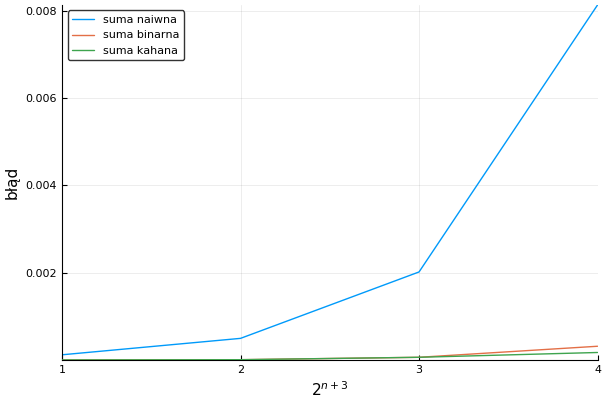
\includegraphics[scale=0.4]{wykres1}\\
    Rysunek 1. 32 bity, $[2^3,2^7]$
\end{center}
    Co ciekawe kiedy powiększamy potęgę dwójki o jeden, to błąd sumowania naiwnego rośnie cztero-krotnie.
    \subsection{Wyznacznik sumowania}
    W rozdziale \ref{uwarunkowanie} pokazaliśmy jaki jest wzór na uwarunkowanie zadania. Korzystając z niego został przeprowadzony następujący eksperyment
    $$  
        X = 2^{17} \text{ losowych liczb, } \forall{x} \in X \hspace{0.3cm} -50 < x < 150
    $$
    \\
    W tabelce przedstawiono wartości błędów w obliczeniach poszczególnych algorytmów w arytmetyce pojedyńczej precyzji(\textit{float}), w których wartośc wyznacznika jest znacząco różna
    \begin{center}
        TABLICA 4.
        \end{center}
    \renewcommand{\arraystretch}{1.3}
    \begin{center}
        \begin{tabular}{|c|c|c|c|} \hline 
            \thead{Wyznacznik} & \thead{Sumowanie \\ naiwne} & \thead{Sumowanie\\ binarne} & \thead{Sumowanie\\ kahana} \\ \hline
            26.873972 & 1.540447e-03 & 6.908958e-07 & 0.000000e+00 \\ \hline
            1.0001979 & 6.239437e-02 & 1.056283e-04 & 0.000000e+00 \\ \hline
        \end{tabular}
    \end{center}
    
    Pokazuje ona, że błąd wyniku rzeczywiście jest podatny na wyznacznik zadania. Chociaż w obu przypadkach
    losowaliśmy liczby z tego samego przedziału, to zarówno dodawanie binarne jak i naiwne otrzymały znacząco gorszy wynik 
    kiedy wskaźnik zadania był duży.
    \subsection{Wnioski}
    W rozdziale \ref{Testy} omówiony został problem dodawania oraz jak go naprawić. Dodając do tego testy
    można wywnioskować, że w celu zwiększenia dokładności, najlepiej jest zwiększyć precyzję. 
    Zarówno w tabeli 1,2 jak i 3 przy użyciu podwójnej precyzji (\textsl{double}) wyniki uległy 
    znaczącej poprawie. Jeśli nie jesteśmy w stanie użyć lpeszej pracyzji, to można dane posortować rosnąco. Z tabeli 2
    widać, że nawet przy losowych danych jesteśmy w stanie w ten sposób zwykle uzyskać nieco lepsze wyniki. 
    Dla najlepszych rezultatów należy jednak zaimplementować algorytm binarny albo jeden z wariantów algorytmu kahana.
    W niemalże każdym przypadku sprawują się one lepiej niż naiwne dodawane, a w połączeniu z lepszą precyzją uzyskują bardzo małe błędy. 
    Ale z tych trzech algorytmów zdcydowanie najlepiej sprawiło się sumowanie metodą kahana.
    W większości eksperymentów zwracał on bezbłędne wyniki.   
    \section{Podsumowanie}
    Przeprowadzone eksperymenty oraz dowody pokazują, że proste dodawanie liczb
    nie jest takim trywialnym problemem. Przy doborze odpowiednich danych jeśli nie użyjemy odpowiedniego algorytmu, to możemy nawet nie zauważyć, że
    otrzymujemy zły wynik i coś jest nie tak. Dlatego lepiej zawsze implementować lepszy algorytm taki jak kahana, bo
    gwarantuje on najlepszą dokładność i niezawodność.
\begin{thebibliography}{9}
    \itemsep2pt
    \bibitem{KH} A. Klein, A generalize Kahan-Babuska-Summation-Algorithm, 2005.
\end{thebibliography}    
\end{document}


